\chapter{Requirement analysis}\label{chapters:analysis}

This chapter summarizes the expectations for the application in the form of requirements. The requirements are analyzed in this chapter, and in the following chapter, the solution is proposed with a focus on a formal description of the framework.

\bigskip

As \textbf{stakeholders} we would consider data analysts, programmers, or at least people interested in the area of data-modeling, as the typical use-case of the application is (i) to design schemas for a large system of interconnected subsystems or modules, or (ii) to design a recommendation for publishing data. Both these use-cases were described in the introduction of this chapter.

Because of the stakeholders' knowledge in the area of data modeling, we may keep the UI of the application more technical as the intent of all operations may be intuitive for them. Nevertheless, the basic functionality does not require advanced knowledge in the mentioned fields, so we propose an "expert mode." User will be asked whether he or she feels to be an expert in the area, which would make available more advanced features of the application while keeping the UI simple for those interested in the basics of data modeling.

\bigskip

\begin{requirement}
A user shall be able to easily derive a \textbf{general schema} structure from the existing ontologies and then translate the structure into different known schema languages, such as JSON Schema, XSD and CSVW Schema and it shall be possible to add support for others easily.
\label{requirement:general-schema}
\end{requirement}

The basic idea behind this requirement was already explained in the introduction chapter. From an ontology, which specifies the relations between things from a real world, it should be possible to easily select relations and things that will describe a schema. The schema then describes a structure of data that represents those things.

\begin{figure}[h!]\centering
  \begin{tikzpicture}
      %Nodes
      \node[ontology] (ontology) at (0,0) {Ontology};

      \node[general-schema] (schema1) at (-3.5,-1.5) {General schema 1};
      \node (psmDot) at (0,-1.5) {...};
      \node[general-schema] (schemaN) at (3.5,-1.5) {General schema N};

      \node[schema,align=center] (xml1) at (-5.5,-3) {XML\\schema};
      \node[schema,align=center] (json1) at (-3.5,-3) {JSON\\schema};
      \node[schema,align=center] (csv1) at (-1.5,-3) {CSV\\schema};

      \node (psmDot) at (0,-3) {...};

      \node[schema,align=center] (xmlN) at (1.5,-3) {XML\\schema};
      \node[schema,align=center] (jsonN) at (3.5,-3) {JSON\\schema};
      \node[schema,align=center] (csvN) at (5.5,-3) {CSV\\schema};

      %Lines
      \draw[-latex] (ontology) -- (schema1);
      \draw[-latex] (ontology) -- (schemaN);

      \draw[-latex] (schema1) -- (xml1);
      \draw[-latex] (schema1) -- (json1);
      \draw[-latex] (schema1) -- (csv1);

      \draw[-latex] (schemaN) -- (xmlN);
      \draw[-latex] (schemaN) -- (jsonN);
      \draw[-latex] (schemaN) -- (csvN);
  \end{tikzpicture}
  \caption{Diagram showing the core workflow behind the data modelling from an ontology. User can create general schemas (blue rectangles) from the ontology from which are created traditional data schemas, such as XSD, CSV Schema or JSON schema.}
\end{figure}

\smallskip

We aim to design a model for a general schema that can describe most of the serialization data formats. This model will be used as a mapping from the ontology to the desired schema. The model must be robust enough to support different formats, as we want to use the same for all of them.

There are many formats for data exchange, the most famous being JSON, XML, CSV/TSV, and RDF. The formats can be categorized into the following categories based on the model of the structure:
\begin{itemize}
    \item \textbf{Hiearchical model} stores data in a tree-like structure, having one root thing with properties that may recursively contain other things. It was one of the most common models for data serialization in the past few decades as it was easy to understand and interpret. XML and JSON are examples of formats that use this model.
    \item \textbf{Relational model} uses a set of tables to store data. Each table represents a sequence of similar things, each on one row with columns as properties. Rows may point to rows in other tables to link data. The relational model is also famous for its simplicity in CSV and TSV files which can be easily parsed.
    \item \textbf{Graph model} represents data in general graph structure with nodes and edges. RDF (Resource Description Framework) became a popular format using the graph model, where nodes usually represent things or literal values and edges connect them as properties.
\end{itemize}

As our primary intent is to support JSON and XML, we will use the first type of model to represent data in our general format. The translation from that format to individual schemas in the hiearchical model would be implicit.

Supporting translation from the general schema, which is in the hierarchical model, to the formats in the relational and graph models should be possible in a limited way\footnote{That means we may not be able to reverse translation from specific schema to the general schema or it may not be possible to use the full power of the given specific schema. However, this is not important to us as our target is support for basic use-cases.}, which is sufficient and follows the requirement to have one general schema.

The graph model is not even necessary to generate as we use the ontology that is already in the graph model; hence we can use the ontology directly as the schema to validate our data.


%==============================================================================%
\section*{Analysis of the formats}

We will analyze the standard formats to properly design a user interface for the schema modeling and the underlying general schema model capable of describing those formats.

\smallskip

\textbf{JSON (JavaScript Object Notation)} is a simple format with two complex data types: objects and arrays. The objects represent data in key-value pairs, with values that can have any type, including other objects and arrays. Arrays then represent lists, and both arrays as objects may be in the root of the document tree. Semantically, objects represent things, with their values as properties.

\textbf{XML (Extensible Markup Language)} is similar to JSON as both formats are hierarchical. XML tags wrap parts of the document representing either things or properties of things and can be nested similarly to the JSON format. In contrast to JSON, XML tags can have attributes.

\begin{figure}[h!]\centering
    \begin{subfigure}[b]{.45\textwidth}
\begin{Verbatim}[commandchars=\\\{\}]
\{
  "id": 3758,
  "title": "Chair",
  "variants": [
    \{
      "title": "Black",
      "price": 200,
      "color": "black"
    \},
    \{
      "title": "White",
      "price": 200,
      "color": "white"
    \}
  ]
\}
\end{Verbatim}
        \caption{JSON document - braces {\tt\{\}} wraps object and brackets {\tt[]} wraps array}
      \end{subfigure}\hfil%
      \begin{subfigure}[b]{.45\textwidth}
\begin{Verbatim}[commandchars=\\\{\}]
<Good id="3758">
  <title>Chair</title>
  <Variant>
    <title>Black</title>
    <price>200</price>
    <color>black</color>
  </Variant>
  <Variant>
    <title>White</title>
    <price>200</price>
    <color>white</color>
  </Variant>
</Good>
\end{Verbatim}

\vfill

        \caption{XML document - {\tt<Good>} tag serves as a class wrapper, whether {\tt<title>} has a property meaning}
      \end{subfigure}
    \caption{Comparison of JSON and XML format both showing data about the same chair.}
    \label{analysis/xml-json}
\end{figure}

As seen from \autoref{analysis/xml-json}, the XML format is more complex, as it supports tag attributes (see the \verb|id="3758"| attribute), and arrays can be written in two distinct ways. We can place items of the array directly in the parent container, as we can see with the \verb|<Variant>| tag, or we can wrap them into another container for clarity (for example, into \verb|<variants>| tag).

\smallskip

JSON Schema is a JSON document describing the data structure we can expect in JSON documents. For this part of the thesis, it is sufficient to know that the schema defines which root object we can expect and a set of allowed properties and their types for each object.

Suppose we have chosen a structure very similar to JSON Schema to be our general structure format. We are interested only in how it describes the document's structure, not its representation. Because JSON is simpler than XML, we can use our model to describe only simple XML documents as we are missing constructs that would describe advanced XML features.

For example,
object property {\tt x} with primitive value {\tt y} would represent an XML tag {\tt <x>y</x>}; if {\tt y} is an object, we will recursivelly apply this rule.
Object property {\tt x} with an array of {\tt y\textsubscript{i}}  would represent multiple XML tags {\tt<x>y\textsubscript{1}</x><x>\nobreak\hfil\penalty0 \hfilneg y\textsubscript{2}</x>...<x>y\textsubscript{n}</x>}.
Finally, we will start with the root tag, which was {\tt <Good>} in our case.

To describe and distinguish between more advanced XML features, we would need to add XML-specific options to our model, such as:
\begin{enumerate}
  \item For every object property with a primitive value, there should be an option that the given property become an attribute of the parent tag. For example, the \verb|id| property of the chair may be either the attribute \verb|id="3758"| of the parent, or the full tag \verb|<id>3758</id>| inside the parent.
  \item For every array property, there should be an option that the given list of tags will be wrapped.
  \item XML, compared to JSON, recognizes an order of the elements in the document. This means that we may decide whether we want to enforce the specific order or not, which can also be fixed by another option in the parent.
\end{enumerate}

Comparing structure of JSON and XML once again, we can let a user use the JSON Schema-like structure with optional annotations for advanced XML features. This allows us to have a simple model which is easy to understand and use and can be annotated by other options for specific languages, as we have shown for XML.

\smallskip

\textbf{CSV (Comma-Separated Values)} or TSV stores data in tables. This, unfortunately, means that the structure is completely different than in the case of JSON and XML. Because having a separate schema would cause complications against other requirements, we will analyze whether it is possible to translate our general structure format from a hierarchical model to a relational one.

In the general case, there are existing approaches \cite{10.1145/304181.304220, 10.1007/3-540-45271-0_10} to map hierarchical model to relational. Therefore, we will show only a brief example. Suppose our general structure format contains objects, properties, and arrays. From each object type, we will create a table with columns as properties. Each table must have a primary key so that the tables can be linked together. If the schema contains an array, we will link children to the parent table; thus, array properties will not have a column.

\begin{figure}[h!]\centering
  \begin{subfigure}{.5\textwidth}
    \centering
    \begin{tabular}{ll}\toprule
      id   & title \\ \midrule
      3758 & Chair \\ \bottomrule
    \end{tabular}%
  \end{subfigure}%
  \begin{subfigure}{.5\textwidth}
    \centering
    \begin{tabular}{llll}\toprule
      good-id & title & price & color \\ \midrule
      3758 & Black & 200 & black \\
      3758 & White & 200 & white \\ \bottomrule
    \end{tabular}
  \end{subfigure}
  \caption{Document of two CSV tables representing the same data as in the \autoref{analysis/xml-json}. Left table contains the root.}
  \label{analysis/csv}
\end{figure}

Because all the tables represent arrays, we can not formally convert the schema with an object in the root. We have suppressed this in the \autoref{analysis/csv} simply by wrapping the schema root into the array.

To support CSV documents containing unrelated data, specifically CSV tables, that do not reference each other, we may need to have a schema with multiple roots. Multiple root schemas may be helpful in some advanced data-modeling problems. We will keep the question behind this open as there are not enough use-cases right now.

Although we have not dealt with advanced cases, the model is robust enough for most use cases.

\section*{General schema format}

So far, we have shown that a JSON Schema-like model with format-specific annotations is sufficient for describing a structure of JSON, XML, and CSV documents. In general, we cannot have too strict requirements on the model as some other formats may not require all the information or may be too simple. This pushes us to define the schema in the most elementary way.

\medskip

We will allow only classes to be a root of schemas and instead add an option that the root can be an array. This simplifies the work with the model as we may always expect a class.

Classes then have an ordered list of properties. This is different from JSON, where properties have no order. A property may be an attribute or association. An attribute has a primitive type, such as a string or a number. Association is a property with another class. Because we have forbidden the use of arrays in the root, we omit them entirely as an array of primitive values and classes can be achieved by the cardinality of attributes and associations, respectively. Cardinality is an interval specifying how many values a property can have. $1..1$ is for required properties, $0..1$ for optional, and $0..*$ for arrays.

\smallskip

We can use two different approaches to visualize the model's hierarchical structure. Previous tools \textit{xCase} and \textit{eXolutio} used graph visualization, where nodes were used to show classes and edges to show associations. An alternative approach is to use a textual "bullet list" representation, as the model is \textit{usually} a tree.

The latter approach is easier to understand as the final product is a schema for documents that has a similar "structure" as the representation. It is easier to implement, more compact in size on the screen, and easier to work with on smaller devices. Also, the order of the properties is more intuitive, and we can use more styling options for advanced constructs.\footnote{So far, we have described only a basic schema structure. See other requirements for advanced constructs.} However, in the general case, users may benefit from the graph view if the schema refers to another schema (see the \autoref{analysis/requirement/schema-reference}) multiple times because this can be easily denoted in the graphical interface (see \autoref{analysis/difference-between-graphical-and-hiearchical}).

\begin{figure}[h!]\centering
  \begin{subfigure}{.5\textwidth}
      \centering
      \begin{tikzpicture}[
          squarednode/.style={rectangle, draw=blue!60, fill=blue!5, very thick, minimum size=5mm},
      ]
          %Nodes
          \node[ontology] (root) at (0,0) {root class};

          \node[squarednode] (a1) at (-1.5,-1.5) {association 1};
          \node[squarednode] (a2) at (1.5,-1.5) {association 2};

          \node[ontology] (ref) at (0,-3) {referenced class};

          %Lines
          \draw[-latex] (root) -- (a1);
          \draw[-latex] (root) -- (a2);
          \draw[-latex] (a1) -- (ref);
          \draw[-latex] (a2) -- (ref);
      \end{tikzpicture}
      \caption{Graphical representation}
    \end{subfigure}%
    \begin{subfigure}{.5\textwidth}
\begin{Verbatim}[commandchars=\\\{\}]
{\color{purple!60}root class}
  {\color{blue!60}- association 1} to
      {\color{purple!60}referenced class}
  {\color{blue!60}- association 2} to
      {\color{purple!60}referenced class}
\end{Verbatim}
      \caption{Hiearchical representation}
    \end{subfigure}

  \caption{Figure showing a schema referencing the same subschema twice, essencially creating a cycle in unoriented graph. Two different representations are shown - graph and hiearchical.  The former one shows that both associations refer the same subschema, which later representation can not show.}
  \label{analysis/difference-between-graphical-and-hiearchical}
\end{figure}

Because the main use-case is to generate simple or moderately advanced schemas, the textual approach is preferred. Nevertheless, the graph view might be implemented in the future.

\medskip

As shown in the \autoref{analysis/difference-between-graphical-and-hiearchical}, the schema may be represented as a "bullet list" where each class, association, or attribute is on a separate line. Classes have a list of properties under the class name. Associations point directly to other classes, and, therefore, they can be merged with the class name on a single line. Other attributes, including format-specific, will be on the line next to the item name.

\begin{figure}[h!]\centering
  \begin{Verbatim}[commandchars=\\\{\}]
{\color{purple!60}class \textbf{Good}}
  {\color{blue!60}- attribute \textbf{id}}[1..1]: string
  {\color{blue!60}- attribute \textbf{title}}[1..1]: string
  {\color{purple!60}- association \textbf{variants}}[0..*]: \textbf{Variant}
    {\color{blue!60}- attribute \textbf{title}}[1..1]: string
    {\color{blue!60}- attribute \textbf{price}}[1..1]: number
    {\color{blue!60}- attribute \textbf{color}}[1..1]: string
\end{Verbatim}
  \caption{Proposition for how the general schema may be represented for the example that validates data with the chair.}
  \label{analysis/general-schema-representation}
\end{figure}

It shall be possible to change the order of the properties by dragging them, and options for given items shall be available next to them. Attributes and associations shall be distinguished both by color and supporting graphics. More advanced constructs may have unique styling options to provide more information if necessary.


%%%%%%%%%%%%%%%%%%%%%%%%%%%%%%

\begin{requirement}
    The application shall create supporting documents for the generated schemas.
\end{requirement}

As the application's main goal should be to generate schemas, we also need to create documentation for them, diagrams, and examples. This requirement has already been described in the introduction chapter.

Schemas use things from ontology, a complex graph of different concepts and relations. To let users better understand it, a diagram of a subset of the ontology used by the given schema may be extremely beneficial. % todo jeste se na to podivat

For the schema in the \autoref{analysis/general-schema-representation}, Figures \ref{analysis/xml-json} and \ref{analysis/csv} are examples that can be automatically generated. This would require additional knowledge from the ontology as the application needs to understand that the title should be a buyable item and the price should correspond to the item's actual price. % todo splitnout a dat do future requirements

%%%%%%%%%%%%%%%%%%%%%%%%%%%%%
\begin{requirement}
    \label{requirement:ontologies-on-the-web}
    As many ontologies are located on the web in formats like OWL (Web Ontology Language), RDFs (RDF Schema), UFO (Unified Foundational Ontology), etc., the application shall support reading them.
\end{requirement}

It may seem that designing the ontology directly in the tool is beneficial because a user does not need to use other tools, and the application may already build the schema, which is feedback to the user. This approach was used in tools \textit{xCase} and \textit{eXolutio} as can be seen in the \autoref{fig:exolutio} in the left panel. However, this approach has the following drawbacks:

\begin{enumerate}
    \item Designing an ontology is a well-defined problem. There are many great and time-proven tools we could not cope with.
    \item Even if the ontology will be used just to generate the schemas, it may be worthy of publishing it anyways as others may benefit from it.
    \item It is better to split a complex problem into smaller ones.
\end{enumerate}

On the other hand, not having direct access to the ontology, as it will be on the web, has the following impacts:

\begin{enumerate}
    \item The ontology may \textbf{not always be available}. Unavailability should not forbid us from generating the schemas and making minor changes to them if those changes are not directly related to exploring the ontology.
    \item The concepts in the ontology may \textbf{point to another ontology} according to Linked Open Data principles.
\end{enumerate}

For the reasons above, the preferred workflow is designing the ontology separately in the external tool, publishing it on the web, and then modeling the schema in the application. There is the \autoref{requirement:pim-editing} later in the text specifying that a user can do modifications in the application. This is not inconsistent with the statements as it deals with minor changes instead of defining a complete ontology.

The term ontology has already been defined in the introductory chapter, and we will formally define its specific requirements in the next chapter.

It shall be easy to implement support for other types of ontologies, and all of them shall be linkable according to LOD principles.

\section*{Format of the ontology}

In the requirement above, several different formats were proposed for the ontology. This section will analyze the minimal requirements for any ontology format and how we will treat additional information in them. Because the core goal is to design schemas, we will start with a proposed model from the \autoref{requirement:general-schema}. The schema consists of classes and their properties. A class corresponds to a thing from real life. An attribute is a literal that belongs to the given class only. An association, on the other hand, is a link between two (not necessarily different) classes. From this point of view, the association is an independent entity.

Associations are usually oriented, and some ontologies may specify a title and a description for a reverse direction. For example, in RDFS, the association (or property in RDFS terminology) is an entity of type {\tt rdf:Property} having domain and range classes and a title and description. Therefore, it only describes the forward direction. We can, of course, create a property in the other direction as well, but there would not be a connection between a forward and a reverse direction. Hence we would not know those are semantically the same properties. UFO (Unified Foundational Ontology), as an example of more complex ontology, introduces relators. Relators are relationships between two or more things connected by mediation. The mediation can be described, giving us a way to describe both directions differently.

Although the latter approach is more complex, using simple concepts for associations may be disadvantageous because of the abovementioned reason. Therefore, we will follow the pattern of UFO and any other simpler ontologies, such as RDFS, will not have the reverse direction described.

\smallskip

An ontology in the context of this requirement is a set of classes that have attributes. Associations then connect two classes together. The connected classes may not be from the same ontology.

As some formats specify ontology in a more complex way, the application may use the additional information to better design the schema. This statement is better defined in the next chapter.

\begin{figure}[h!]\centering
  \centering
  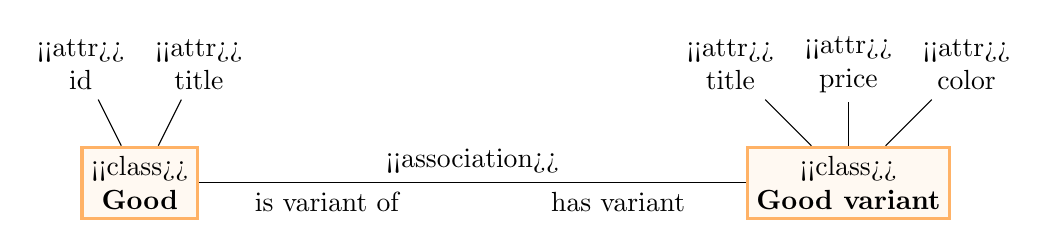
\begin{tikzpicture}[
    class/.style={shape=rectangle, draw=orange!60, fill=orange!5, very thick, minimum size=5mm,align=center},
    attribute/.style={align=center},
  ]
    \node[class] (good) at (0,0) {<<class>>\\\textbf{Good}};
    \node[class] (variant) at (9,0) {<<class>>\\\textbf{Good variant}};

    \node[attribute] (a11) at (-.75,1.5) {<<attr>>\\id};
    \node[attribute] (a12) at (.75,1.5) {<<attr>>\\title};

    \node[attribute] (a21) at (7.5,1.5) {<<attr>>\\title};
    \node[attribute] (a22) at (9,1.5) {<<attr>>\\price};
    \node[attribute] (a23) at (10.5,1.5) {<<attr>>\\color};

    \draw (good) -- (a11);
    \draw (good) -- (a12);

    \draw (variant) -- (a21);
    \draw (variant) -- (a22);
    \draw (variant) -- (a23);

    \draw (good) -- node[pos=0.225,below]{$\blacktriangleleft$ is variant of} node[above]{<<association>>} node[pos=0.775,below]{has variant $\blacktriangleright$} (variant);
  \end{tikzpicture}

  \caption{Schematic diagram of an ontology which could be used for the schema from the \autoref{analysis/general-schema-representation}.}
\end{figure}

% todo popis, jak by mela ontologie vypadat na zaklade toho schematu. Jakou by mela mit strukturu a co musi obsahovat

% mozna ze to je jak uml

%%%%%%%%%%%%%%%%%%%%%%%%%%%%%%%%%%%%%%%%%%%%

\begin{requirement}
    The application shall support generating transformations between different data conforming to supported schemas and RDF representation.
\end{requirement}

Data transformation was also introduced at the beginning of this thesis. Generally speaking, \textbf{data transformations} are used to convert data (not schemas, but data that conforms to given schemas) from one schema to another without changing its meaning.

One example may be to convert CSV to a JSON array of objects, where each object represents a row in the CSV. There are plenty of online tools to do it, but they do not understand the context of the data. Because both schemas were designed in the tool, we may exploit the knowledge of the mapping to the original ontology and correctly map columns from CSV to the fields in a JSON object.

In the context of this tool, transformation means both (i) transformation between different schemas under the same general schema and (ii) between different general schemas, if possible. As an example of the second case, we may have two general schemas for the same thing, where one is simpler than the other. For example, we may have the schema from the \autoref{analysis/general-schema-representation} and similar with more attributes and associations, possibly with a different order of properties and labels. It is then possible to convert data from the more complex schema to the simpler one by losing information. If default values are provided, or additional properties are optional, the transformation in the other direction should also be possible.

\medskip

Regarding the transformation process, there are plenty of ways how to transform data:
\begin{enumerate}
    \item Data engineers use \textbf{Python} with support of many formats using libraries. In this case, the transformation would mean a generated Python script with a pre-defined interface that takes data from one format and outputs in another. Depending on the use case, the script may be configurable (besides the possibility to configure the generation of transformation itself).
    \item There is \textbf{XSLT} (Extensible Stylesheet Language Transformations) language for transforming between XML documents or from XML to XML-like, plain-text or CSV documents. XSLT is an XML document that can be executed with an input document by an XSLT processor producing a resulting document. One disadvantage is that the input document must be in XML format; hence it can not be used alone for bi-directional JSON and CSV transformation.
    \item There are mapping tools such as RML \cite{dimou2014rml} (RDF Mapping Language) designed explicitly for mapping purposes. RML maps common serialization frameworks such as XML, CSV, and JSON to RDF from a set of rules written in RDF. The translation mechanism is similar to the XSLT.
\end{enumerate}

Although RML is a ready-to-use solution with support for all three technologies, it requires its own toolchain for transformation. In contrast, XSLT is well-known technology among people working with XML and is widely supported. Therefore, our primary concern will be to implement XSLT for XML while keeping the RML for later.

Similar to the translation of a human text, there are two approaches. Either create transformation for each pair or have one standard format where all others can be transformed and vice versa. The latter approach requires only one transformation for each new format added and is easier to debug, as there is a middle format. Because the schemas are built from ontologies whose primary source is RDF, we will exploit this and have RDF as the middle format, which is another format we can transform data to.

\medskip

We categorize two types of transformations - lifting and lowering. Lifting is a process of converting semi-structured data such as JSON, XML, or CSV into RDF. Lowering is the opposite process, and by combining them, we can achieve a transformation between various formats. That means that even if we want to transform XML to CSV, which would be possible by a single XSLT document for simple structures, we would need to execute two transfomations.

\begin{figure}[h!]\centering
    \begin{tikzpicture}
        %Nodes
        \node[ontology] (ontology) at (0,0) {Ontology};

        \node[artefact,align=center] (rdf) at (3,-1.5) {RDF documents};

        \node[general-schema,align=center] (schema1) at (-3,-1.5) {General\\schema};

        \node[schema,align=center] (xml1) at (-4,-3) {XML\\schema};
        \node[schema,align=center] (json1) at (-2,-3) {JSON\\schema};

        \node[artefact,align=center] (xml_document) at (1.5,-3.5) {XML\\document};
        \node[artefact,align=center] (json_document) at (4.5,-3.5) {JSON\\document};

        \draw[-latex] (rdf) -- node[above,anchor=south west,align=left] {conforms} (ontology);

        \draw[-latex] (ontology) -- (schema1);
        \draw[-latex] (schema1) -- (xml1);
        \draw[-latex] (schema1) -- (json1);
        \draw[-latex] (xml_document) to[bend left] node[below] {conforms} (xml1);
        \draw[-latex] (json_document) to[bend left] node[below] {conforms} (json1);

        \draw [->,line width=1pt, transform canvas={xshift=-1.25em}] (xml_document) -- (rdf);
        \draw [->,line width=1pt, transform canvas={xshift=-0.5em}] (rdf) -- (xml_document);

        \draw [->,line width=1pt, transform canvas={xshift=0.5em}] (json_document) -- (rdf);
        \draw [->,line width=1pt, transform canvas={xshift=1.25em}] (rdf) -- (json_document);

        \node[rectangle,fill=white] at (3,-2.35) {lifting and lowering};
    \end{tikzpicture}
    \caption{Example of data transformation. An XML document that conforms to XML schema may be lifted to RDF representation, which conforms to the ontology. The RDF can then be lowered to another format.}
\end{figure}


%%%%%%%%%%%%%%%%%%%%%%%%%%%%%%%%%%%%%%%%%%%%%%

\begin{requirement}
  It shall be possible to refer to other schemas to use them as building blocks for larger ones. Schema reference shall be treated as a reference on the resulting schemas and documentation as well.
  \label{analysis/requirement/schema-reference}
\end{requirement}

Referencing other schemas is crucial for advanced use-cases where it is essential to split large schemas into smaller blocks that can be published and used separately.

For most schema languages, it should be sufficient to refer to the other schema as is. For example, in JSON, we can use the \verb|$ref| keyword with a path to the referenced schema. On the other hand, data transformations might not always be able to handle this approach. Hence having a full copy of the schema might be necessary. Referencing a schema would thus require access to all data of its specification.

To avoid problems with tracking references and knowing which data specification needs to be loaded to generate artifacts properly, a user would need to set explicitly that a given \textbf{data specification is being reused}. Similar to the requirement with the ontology, we do not require that the reused data specification be always available.\footnote{See the requirement X for context.} The application shall work even if the data specification is not available at the moment if the presence of the specification is not required directly - such as for creating a new reference or generating artifacts that depend on it.

\begin{figure}[h!]\centering
  \begin{tikzpicture}
      \node[data-specification,align=center] (ds1) at (-3,0) {Data specification 1};
      \node[data-specification,align=center] (ds2) at (3,0) {Data specification 2};

      \node[general-schema,align=center] (s11) at (-4.5,-1.5) {General\\schema};
      \node[general-schema,align=center] (s12) at (-1.5,-1.5) {General\\schema};
      \node[general-schema,align=center] (s21) at (3,-1.5) {General\\schema};

      \draw[-latex] (ds1) -- (s11);
      \draw[-latex] (ds1) -- (s12);
      \draw[-latex] (ds2) -- (s21);

      \draw[-latex,densely dotted] (ds1) -- node[above] {reuses} (ds2);
      \draw[-latex,densely dotted] (s12) -- node[above] {refers} (s21);
  \end{tikzpicture}
  \caption{Example of reusing of specifications. All schemas from reused specification become available to refer from local schemas. Only the root of the schema may be refered.}
\end{figure}


%%%%%%%%%%%%%%%%%%%%%%%%%%%%%%%%%%%%%%%%%%%%%%%%%%%%%%%%%%%%%%%%%%%%%%%%%%%%%%%

\begin{requirement}
  List of supported schemas, transformations, documents, and other files generated from the general schema shall be easily expandable so that the application can be adapted to different use-cases.
\end{requirement}

Generation of schemas is robust enough to be used in every common scenario, therefore we do not expect that user may want to intervene the process besides the standart configuration, such as indentation, using of comments, or a default language.

On the other hand, documentation is very vague concept that neither we have properly specified. Sometimes a simple Markdown documentation may be sufficient, while elsewhere user may require a strict format of multiple documents in HTML.

Transformations have similar issue. There are multiple ways and technologies that transform data between different schemas. We have already mentioned transformation throught RDF format, either by RML, or custom scripts, such as XSLT for XML. For more demanding user, it is even possible to create transformation scripts between pairs of technology, such as between XML and CSV.

We will expose a way user can register his/her own generator that can create a set of files in a filesystem from the given schema.

Generators may use others to modify their results, further expends them, or just link them.
% Pozadavek na OFN?

\section*{Artifacts}

There is little difference between generated schemas, data transformations, documentation, and other output files. Based on the general schema and provided configuration, if any, the application shall create a set of files that can either be published on the Web or stored in the file system. All the generated files will be denoted as \textbf{artifacts} and are created by the \textbf{generators}.

We will distinguish two types of artifacts. (i) The \textbf{specification artifacts} does not depend on a concrete schema but uses the whole specification. Documentation may be an example of a specification artifact because it generates a single document concerning all the schemas. Of course, this still depends on user requirements, and scheme-specific documentation is possible. (ii) The \textbf{schema artifacts} are bound to concrete general schema and are used to generate transformations or the schema documents.

Artifacts may reference other artifacts. For example, documentation may be the front page of the whole structure, having links to other documents, schemas, images, etc.

\begin{figure}[h!]\centering
  \begin{tikzpicture}
      \node[data-specification,align=center] (ds1) at (-3,0) {Data specification};

      \node[general-schema,align=center] (s11) at (-4.5,-1.5) {General\\schema};
      \node[general-schema,align=center] (s12) at (-1.5,-1.5) {General\\schema};

      \node[artefact,align=center,cascaded] (sa1) at (-7.5,-1.5) {Specification\\artefacts};

      \node[artefact,align=center,cascaded] (sa11) at (-4.5,-3) {Schema\\artefacts};
      \node[artefact,align=center,cascaded] (sa12) at (-1.5,-3) {Schema\\artefacts};

      \draw[-latex] (ds1) -- (s11);
      \draw[-latex] (ds1) -- (s12);
      \draw[-latex] (ds1) -- (sa1);

      \draw[-latex] (s11) -- (sa11);
      \draw[-latex] (s12) -- (sa12);
  \end{tikzpicture}
  \caption{Schemas, documentation, and other generated files are artefacts. Artefact are either schema-specific, that are generated for every schema, or specification-specific for a given data specification.}
\end{figure}


%%%%%%%%%%%%%%%%%%%%%%%%%%%%%%%%%%%%%%%%



% Necaskeho pozadavek na OR a hierarchii
% https://github.com/mff-uk/dataspecer/issues/95

\begin{requirement}
    It shall be possible to easily add more specific classes to the general schema that extends the base class in a way that data, that conforms the resulting schemas, may contain either the base class, or one of its specialization.
\end{requirement}

\begin{showcase}
    We will start directly with an example. Suppose, that the warehouse also distributes foods besides the general goods. Food is of course type of good, but for storing purposes, it may have additional attributes, such as \textit{storing temperature}. When designing a schema that contains goods anywhere


\end{showcase}

This requirement impacts the application on two different levels. First, the general schema model has to have constructs to represent the required problem and all generators shall understand them and generate a schema that corresponds to the intended result.

Generaly speaking, inheritance is a complex concept, that can be expressed in more simple way. Unfortunatelly, to make this pleasible for a user, we need to represent some things % such as association to class

% Analyza co vsechno se da udelat, co bude privetive a co ne. Rozeberu to na zakladni OR a include.




\section{Future requirements}

Following requirements in this section are analyzed and may have an impact on the final model that will be discussed in the next chapter. But due to its complexity, full implementation and analysis will be kept as authors future work and this thesis cover only the necessity to not introduce a technical debt.

%%%%%%%%%%%%%%%%%%%%%%%%%%%%%%%%%%%%%%%%%%%%

\begin{requirement}
  \label{requirement:pim-editing}
  The approach from previous tools of creating the ontology directly in the application is not required, but there should be support for \textit{some} modifications.
\end{requirement}

As stated in the \autoref{requirement:ontologies-on-the-web}, the preffered way is to create a complete ontology externally and keep it up-to-date and valid against requirements of all involved parties. But it is hard to always follow all the rules, especially when doing experiments, or small errors need to be fixed.

Allowing such changes must be made carefully, as it may interfere with some mechanisms.
\begin{enumerate}
  \item If the ontology changes, the local overwrites may need to be changed as well, otherwise may become invalid. Overwritten data may get removed or moved elsewhere. Evolution mechanism hence must work with the overwrites as well.
  \item Moreover, the overwriten data may change, which can lead to two scenarios. Either user wishes to keep the local version as if nothing happend, or he/she may want to discard the local version as the new version fixes the issue that caused the modification in the first place.
\end{enumerate}

This issue is too complex and due to the nature of the requirement, it must be solved directly in the application. We keep the question behind this problem partially open and focus only to simple modifications, as this will cover most use-cases.\footnote{From our specific use-case on the Semantic government vocabulary (SGOV), most of the changes consist of adding a missing cardinality or fixing labels and descriptions.}

\begin{requirement}
    It shall be possible to perform a top-down evolution of schemas and other documents from an ontology. The evolution shall be automatic, if possible, and shall also transorm the data that conform the given schemas. The application shall also deduce the changes from an ontology that does not support versioning.
\end{requirement}

Schema evolution is a large topic with many theoreticall issues.

% popis evoluce, priklady


%%%%%%%%%%%%%%%%%%%%%%%%%%%%%%%%%%%%%%%%%%%%%%%%%%%%%%%%%%%%%%%%%%%%%%%%%%%%%%%%

\begin{requirement}
    As there shall be a support for data transformations between different schemas, the data transfomations shall respect various ontology alignments to transform data between different ontologies. Alignments shall be created also during user modification of the ontology, between the modification and the original ontology.
\end{requirement}

\textbf{Alignment} as defined in TODO is a set of relations between entities \textit{usually} from different ontologies. These relations specify the semantic equivalence between the entities and create a mapping that can transform data from one ontology to another.

There are already well-known RDF predicates that can cover basic alignment. For semantically identicall entities, we may use \verb|owl:equivalentClass| or \verb|skos:exactMatch|. More usefull RDF predicate is \verb|rdfs:subClassOf| for more specific classes representing things.

The later one is already included in the previous requirement TODO. Subclasses (i) reuses attributes and associations from its parent class, but also semantically denotes, that (ii) the subclass can also be treated as "the parent class". The second point is an example of a simple ontology alignment.

\begin{showcase}
    % example with address
\end{showcase}

%%%%%%%%%%%%%%%%%%%%%%%%%%%%%%%%%%%%%%%%%%%%%%


% analyza jak se to bude psat na radek


% todo solid pod
